

\chapter{Results}

In this chapter, we describe the results from our pose and depth experiments. In Chapter 3 we described an unsupervised pipeline for learning depth and visual odometry from monocular imagery. Similarly, in Chapter 4, adapted conventional 2D machine learning techniques to apply 4D image data to learning these tasks. Specifically, we recommended two variants of an algorithm for learning depth and visual odometry from light fields - the first uses all the information from the light field to generate a novel rendering of a single \textit{(U, V)} slice, while the second method uses the known configuration of the camera array to create a rendering of the complete light field. In this chapter, we contrast results for three algorithms - each of the two novel pipelines described in Chapter 4, and the existing monocular approach described in Chapter 3. For the two algorithms that we have suggested, we also evaluate three ingestion methods: focal-stacks, volumetric images, and tiled EPI images. 

First, we evaluate each algorithm's performance in pose-estimation, and demonstrate results for cumulated trajectories for several input-sequences. Subsequently, we'll evaluate the algorithms' performance in depth-prediction and photometric reconstruction. 

\section{Pose Estimation and Visual Odometry}

\subsection{Single-view Reconstruction}
\begin{figure}[H]
    \subfloat[Tiled EPIs]{
        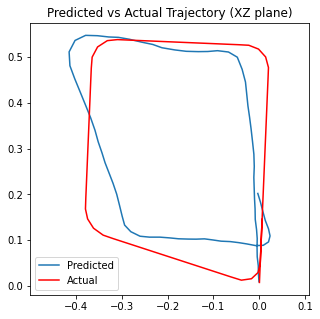
\includegraphics[height=2in]{images/result-examples/pose/trajectories/singlewarp/sw-epi-16.png}
    }
    \subfloat[Focal Stacks]{
        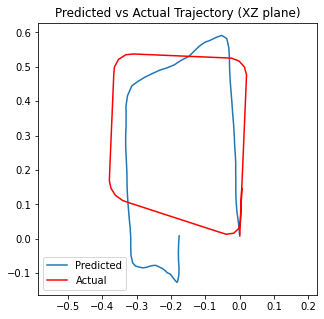
\includegraphics[height=2in]{images/result-examples/pose/trajectories/singlewarp/sw-focalstack-175-16.png}
    }
    \subfloat[Volumetric Images]{
        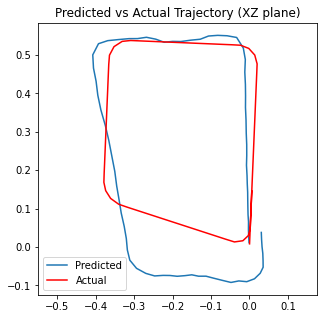
\includegraphics[height=2in]{images/result-examples/pose/trajectories/singlewarp/sw-stack-16.png}
    }\\
    \caption{Estimated and true trajectories for input sequence 16.}
    \setcounter{subfigure}{0}

    \subfloat[Tiled EPIs]{
        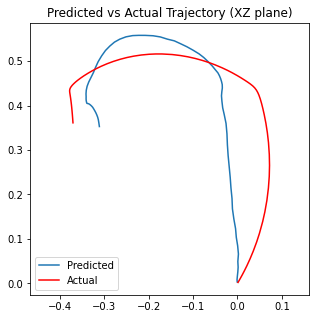
\includegraphics[height=2in]{images/result-examples/pose/trajectories/singlewarp/sw-epi-44.png}
    }
    \subfloat[Focal Stacks]{
        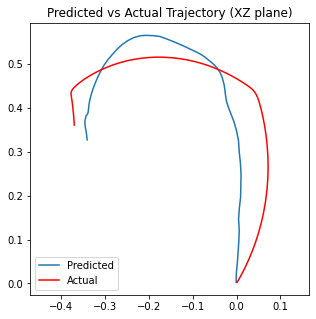
\includegraphics[height=2in]{images/result-examples/pose/trajectories/singlewarp/sw-focalstack-175-44.png}
    }
    \subfloat[Volumetric Images]{
        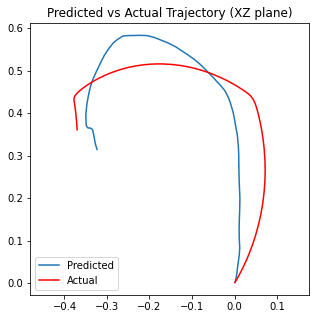
\includegraphics[height=2in]{images/result-examples/pose/trajectories/singlewarp/sw-stack-44.png}
    }
    \caption{Estimated and true trajectories for input sequence 44.}
    \setcounter{subfigure}{0}
\end{figure}

\subsection{Light field Reconstruction}
\begin{figure}[H]
    \subfloat[Tiled EPIs]{
        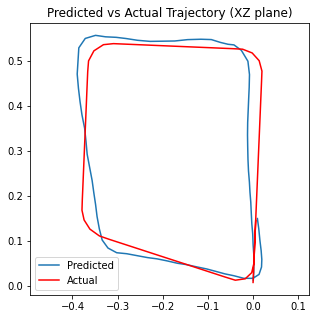
\includegraphics[height=2in]{images/result-examples/pose/trajectories/multiwarp/mw-epi-16.png}
    }
    \subfloat[Focal Stacks]{
        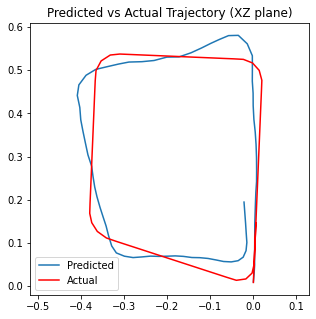
\includegraphics[height=2in]{images/result-examples/pose/trajectories/multiwarp/mw-fs-175-16.png}
    }
    \subfloat[Volumetric Images]{
        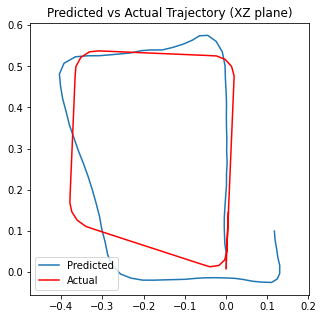
\includegraphics[height=2in]{images/result-examples/pose/trajectories/multiwarp/mw-stack-16.png}
    }
    \caption{Estimated and true trajectories for input sequence 16.}
    \setcounter{subfigure}{0}
    \subfloat[Tiled EPIs]{
        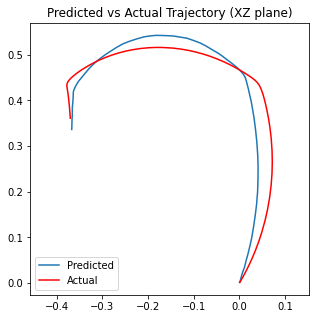
\includegraphics[height=2in]{images/result-examples/pose/trajectories/multiwarp/mw-epi-44.png}
    }
    \subfloat[Focal Stacks]{
        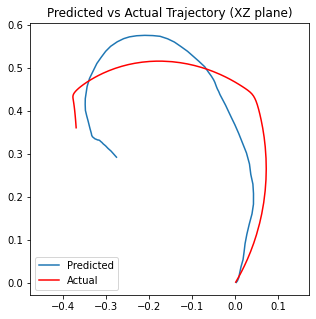
\includegraphics[height=2in]{images/result-examples/pose/trajectories/multiwarp/mw-fs-175-44.png}
    }
    \subfloat[Volumetric Images]{
        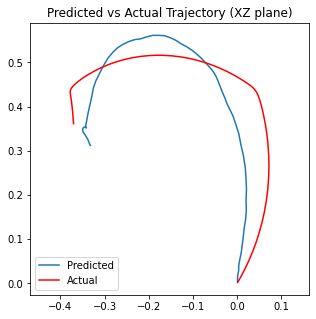
\includegraphics[height=2in]{images/result-examples/pose/trajectories/multiwarp/mw-stack-44.png}
    }
    \caption{Estimated and true trajectories for input sequence 44.}
    \setcounter{subfigure}{0}
\end{figure}


\subsection{Monocular Approach}

\begin{figure}[H]
    \subfloat[Sequence 16]{
        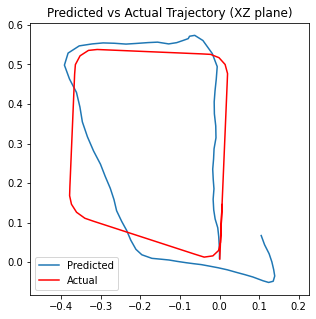
\includegraphics[height=3in]{images/result-examples/pose/trajectories/monocular/monocular-16.png}
    }
    \subfloat[Sequence 44]{
        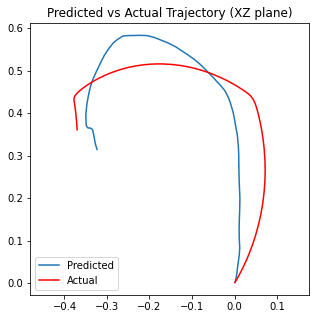
\includegraphics[height=3in]{images/result-examples/pose/trajectories/monocular/monocular-44.png}
    }
    \caption{Estimated and true trajectories using monocular imagery.}
    \setcounter{subfigure}{0}
\end{figure}

\subsection{Light field Reconstruction}


\subsection{Comparison between Pipelines and Summary}

\section{Depth and Photometric Reconstruction}

\subsection{Single-view Reconstruction}
\subsection{Light field Reconstruction}
\subsection{Monocular Approach}

\subsection{Comparison between Pipelines and Summary}





